\documentclass[12pt,a4paper]{article}
\usepackage{fontspec}
\defaultfontfeatures{Mapping=tex-text}
\usepackage{xunicode}
\usepackage{xltxtra}
\setmainfont{FreeSerif}
\setmonofont{FreeMono}
\usepackage{polyglossia}
\setdefaultlanguage{english}
\usepackage{amsmath}
\usepackage{amsfonts}
\usepackage{amssymb}
\usepackage{siunitx}
\usepackage{xcolor}
\usepackage[justification=centering, font={small, sl, color=gray}]{caption}
\usepackage[margin=2.5cm]{geometry}
\usepackage[section]{placeins}
\usepackage{datetime}
\usepackage{hyperref}
\usepackage{indentfirst}
\usepackage{enumitem}

\author{Anas Naïri \and Julien Plante}
\title{Modelisation of ExoMars 2020's network using SystemC}

\setlength{\parindent}{0cm}
\newcommand{\Cpp}{C\texttt{++}}

\begin{document}

\begin{titlepage}


\includegraphics[width = 60mm]{pictures/suai.png}

    \vspace*{\fill}

    \begin{center}
    
        \Huge\bfseries
        Second R\&D project report
        \vskip10pt
        \Large\bfseries
        Modelisation of ExoMars 2020's network using SystemC
        \vskip10pt
        \large
        PLANTE Julien - NAÏRI Anas
        \vskip20pt
        \large
        Saint Petersburg State University of Aerospace Instrumentation.
        \vskip20pt
        
        \vspace*{\fill}
        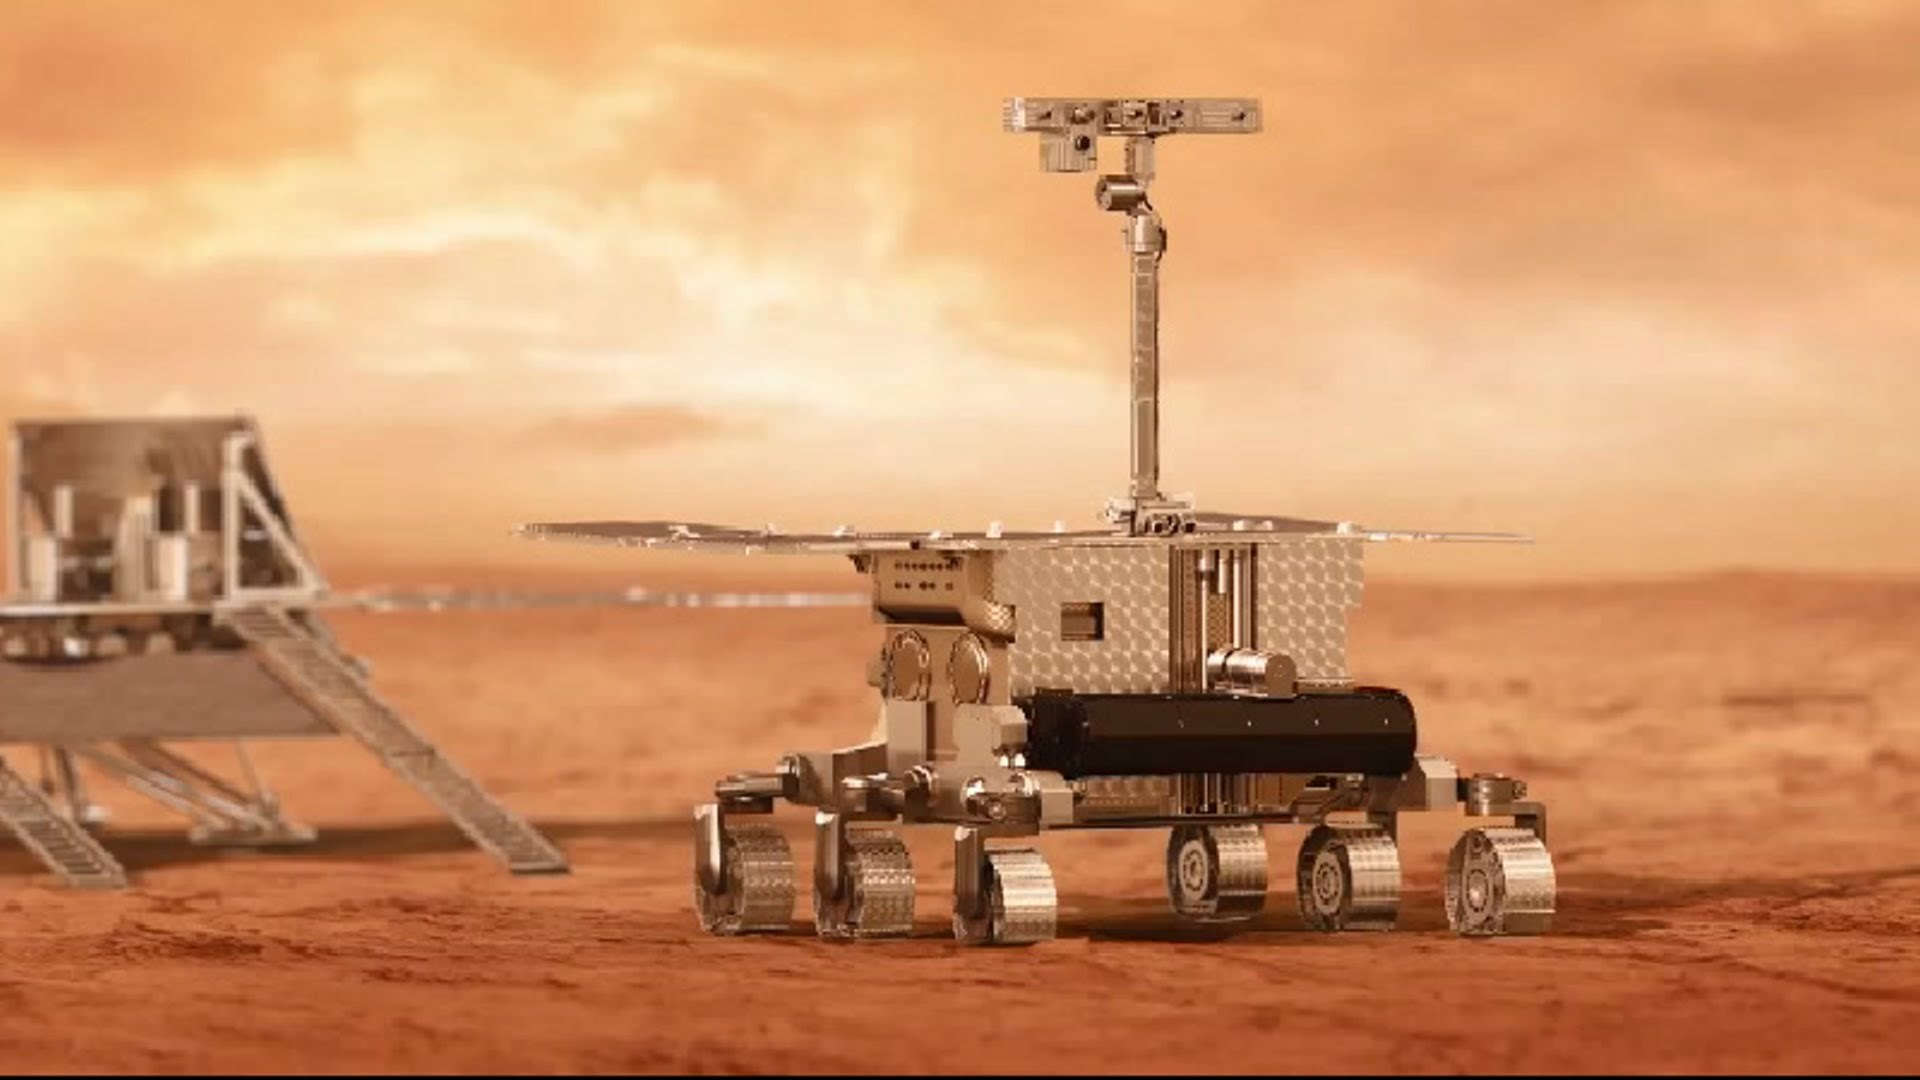
\includegraphics[scale = 0.2]{pictures/Exomars2020.png}
    \end{center}
    
    \vspace*{\fill}

\end{titlepage}

\pagebreak

\tableofcontents

\pagebreak

\section{Task formulation}

\begin{itemize}
    \item Documentation about the ExoMars2020's rover to establish the rover's network structure
    \item Implement the rover's network on SystemC, only the SpaceWire's network layer, channels must handle the speed of transmission and error bit frequency, and devices must generate data into the network and receive data from it
    \item Create a base log-system to record results of the simulation through SQlite
    \item Compare the time modelling between a single model and a parallel model
\end{itemize}

\section{Introduction}

Our second project is a direct continuation with the previous one. To summarize briefly, our first R\&D project was about implementing a SpaceWire's network layer on SystemC, to simulate data sent from Earth and received on a spacecraft.\smallbreak

In fact, this R\&D project, which is to simulate the data-handling network architecture of the ExoMars2020's rover, involves to use a SpaceWire router with a view to interconnecting the multiple scientific instruments. Since the rover uses a lot of cameras to observe, analyse and interpret its environment, then the processing of images taken by these instruments is well needed. In that case, as we can see in the figure below, the rover got a dedicated chip for this kind of process. Data will be sent from equipment, then to the memory, next to the processor which will give instructions to the image processor.\smallbreak

\begin{figure}[hb]
	\centering
    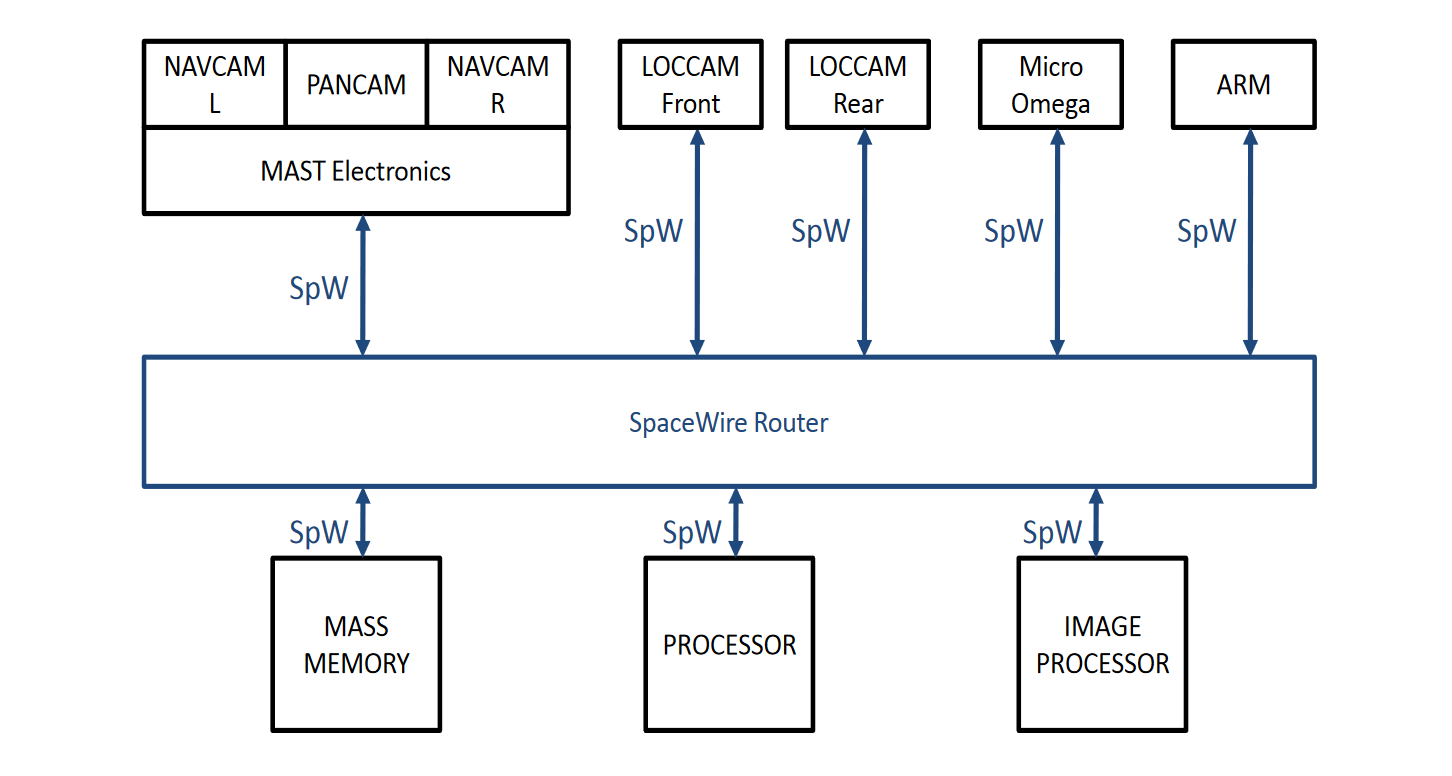
\includegraphics[scale = 0.5]{pictures/data_network_architecture.png}
    \caption{Data-handling structure of ExoMars' rover}
\end{figure}

Consequently, such amount of image processing can be well handled by the use of a SpaceWire router. Because, as we already know, SpaceWire is a good data-handling network which allies high speed of communciation, low powering, and low cost implementation. It is ideal in the case of ExoMars2020, because it needs to connect all equipment to memory and processors. But, in our simulation, we had settled for a simulation involving the scientific instrumentation connected to each other via a SpaceWire router, so it can communicate between them by sending and receiving packets containing the results of a unit. We decided to do so to simplify the implementation, yet, it describes the same behaviour than if we could have put memory and processors. Moreover, ExoMars2020's rover use the RMAP protocol to pass data from equipment to memory then to processors.\smallbreak 

\begin{figure}[hb]
	\centering
    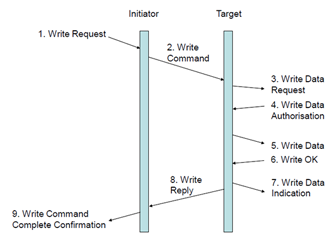
\includegraphics[scale = 0.5]{pictures/RMAP_protocol.png}
    \caption{Description of the RMAP protocol}
\end{figure}



\section{Description of ExoMars2020's rover}

The ExoMars2020 mission has a goal to search evidence of past or present life on the surface and/or subsurface of Mars. Thanks to its rover, it will, in addition, understand more the planet's surface and subsurface, like its origin of formation and the composition of it, by the use of multiple scientific instrumentation as cameras and radars.\smallbreak

\subsection{PanCam}
The PanCam is used to record 2D \& 3D images of the Mars' surface, in order to understand the geological and morphological situation on the planet. In fact, the PanCam is composed of two WAC (Wide Angle Camera), one on the left, the other on the right to have a stereoscopic view of the ground, and a HRC (High Resolution Camera). Also, it operates to produce images in the near infrared and visible wavelength. This device, in synergy with the others, allows the rover to chose the best potential locations site to drill, for example shallow ground that may contains gases or water. The HRC and WAC, both operates with an image resolution of 1024 x 1024 pixels, the first one in RGB, the second with a multispectral filter wheel. The PanCam communicates with packets of 10-bits' data.
\pagebreak

\subsection{ISEM}

The ISEM (or Infrared Spectrometer of ExoMars), as its name means, is an infrared beam that senses the infrared part of the sun's light reflection onto Mars' surface. With this method used on the rocks near of the rover, it obtains the spectrometer of these rocks and then get information about the geological composition of the planet's surface. Indeed, this device helps the rover to chose a potential location to drill in, because the presence of some minerals may indicate good places where to find past life on Mars. It communicates with packets of 16-bits' data.

\subsection{CLUPI}

The CLUPI, or Close-Up Imager, is a high-resolution camera which goal is to take close picture of rocks to be able to detect each details of these ones. Thus, we can know to what type of rock we are seeing or surrounded with, by analyse the texture, the color, the morphology, etc. Also, it will give information about the original context of possible formation of these rocks, like, geological major events that they experienced throughout their existence. Plus, with this kind of close up pictures, we should be able to detect bio-signatures at the surface of rocks. It is permitted because the CLUPI has an image resolution of 2652 x 1768 pixels in RGB. It can take picture in the visible wavelength, with an exposure time of 1024 seconds. It communicate with packets of 14-bits.

\begin{figure}[hb]
	\centering
    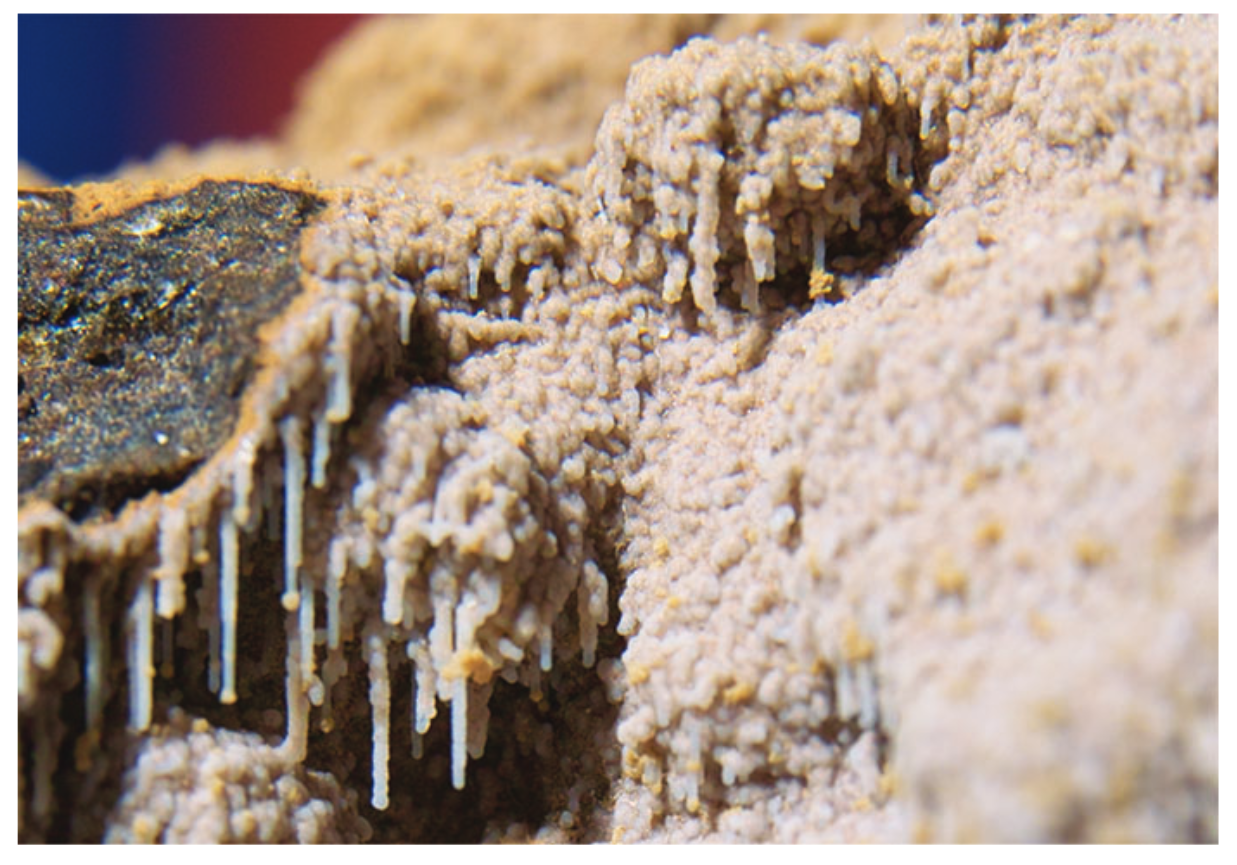
\includegraphics[scale = 0.5]{pictures/close_up_image.png}
    \caption{Close up picture of a rock taken from CLUPI}
\end{figure}

\pagebreak

\subsection{WISDOM}

To find if there are some evidence of the past and present life on Mars, we can search in the subsurface, where organics molecules could be shielded from destructive events. In fact, the WISDOM, or Water Ice Subsurface Deposit Observation on Mars, is a ground penetrating radar which will help to notify and describe the type of the shallow surface that is pointed by this one. If an information about a place in subsurface has been processed as a potentially location of organics molecules, the ExoMars' drill will then dig in it.\smallbreak

In addition, WISDOM is working with others instruments to precise if a place in the subsurface is relevant or not by gathering information from Adron, PanCam and Ma\_Miss. From the Adron, we can obtain information about the composition of a source of water in liquid or ice form. From the PanCam, we get 3D information of the rover's environment, that can help it to better filter locations to dig in. And, because the Ma\_Miss is in the drill, it is in direct contact with the subsurface, thus data from this one are compared with those from WISDOM that will permit to set a 3D map of the subsurface. By the way, WISDOM communicate with other equipment by packets of 16-bits' data.

\subsection{Adron}

The Adron is a detector of radiations of neutrons that are sensed from the subsurface of the planet. With the data from WISDOM, it permits to detect the water distribution in the Mars' subsurface and the presence of certain elements in this water. Then, the combination of the both instruments' data would help to localize the best places to drill in order to find evidences of potential past or present life on or below the surface of Mars. It communicate with packets of 9-bits' data.

\pagebreak
\subsection{Ma\_MISS}
Ma\_MISS, for Mars Multispectral Imager for Subsurface Studies, is a spectrometer located in the drill of the rover, used to determine horizontal and vertical composition of the Martian soil. By illuminating the borehole and analysing the reflected light and its spectrum, it will be able to gather information about the distribution of minerals, especially of water-related ones, to search potential indicators of life.

It will work alongside the three other spectrometers (RLS, MicrOmega, MOMA), being specialised in studying unexposed material, and in collaboration with WISDOM and ADRON to choose interesting drilling location

\begin{figure}[h]
\centering
\includegraphics[scale=.7]{pictures/MaMiss}
\caption{The instrument, located on the drill.\\Credit: SELEX Galileo}
\end{figure}

\subsection{MicrOmega}

MicrOmega is an infra-red spectrometer made to identify composition of Martian soil samples at a grain scale, after their gathering by the drilling system. It is similar as RLS and MOMA in this way, since the three spectrometers will study samples collected by the drill. The infra-red study of the samples is adapted to find evidences of past or present carbon and water presence. 
It uses an infra-red hyper-spectral microscopic imager to acquire the spectrum of a 250$\times$256 pixels square (\char`\~5$\times$5 \si{\milli\metre^2}) for 320 wave length, between 0.95 and 3.65 \si{\micro\metre}. Thus having a maximum of \num{20480000} bytes to transmit.

\subsection{RLS}
RLS uses the Raman effect to find life signatures in Martian soil samples in a non-destructive way.
The measurements carried out by the RLS will be performed as described within the ExoMars Rover Reference Surface Mission, which includes six experiment cycles (with two samples each, one extracted from a surface target and the other at depth) and two vertical surveys (with five samples each extracted at different depths). It generates information about a 2048$\times$512 pixels of 15 \si{\micro\metre}, totalling a surface of approximately 30.7$\times$7.7 \si{\micro\metre^2}, and \num{1048576} bytes.

\subsection{MOMA}
MOMA (Mars Organics Molecule Analyser) is an instrument designed to detect organic molecules in spots of interest detected by the collaboration of RLS and MicrOmega, thus providing extremely precise analysis of Martian environment, and great information about potential origin, evolution and distribution of life on the planet. To do so, it will study samples gathered by the drill, as well as analysing the gases of the Martian atmosphere. It features to modes of operation : Gas Chromatograph-Mass Spectrometry (MOMA GC-MS) and Laser Desorption-Mass Spectrometry (MOMA LD-MS), the first one being used to analyse atmosphere gases, and the second soil samples. No information about size of data produced was found.

\begin{figure}[h]
\centering
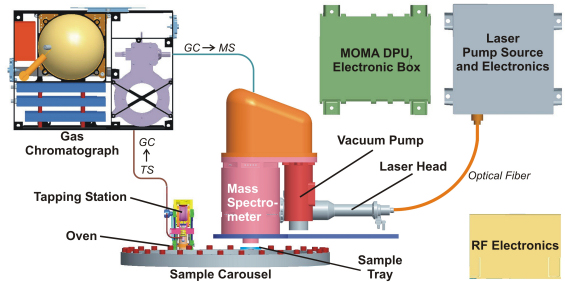
\includegraphics[scale=.7]{pictures/MOMA.jpg}
\caption{The MOMA instrument and its modules.\\Credit: Max Planck Institute for Solar System Research}
\end{figure}

\pagebreak

\section{Model structure and functioning description}
\smallbreak
The final structure of our project looks like this: \smallbreak
\begin{figure}[h]
\centering
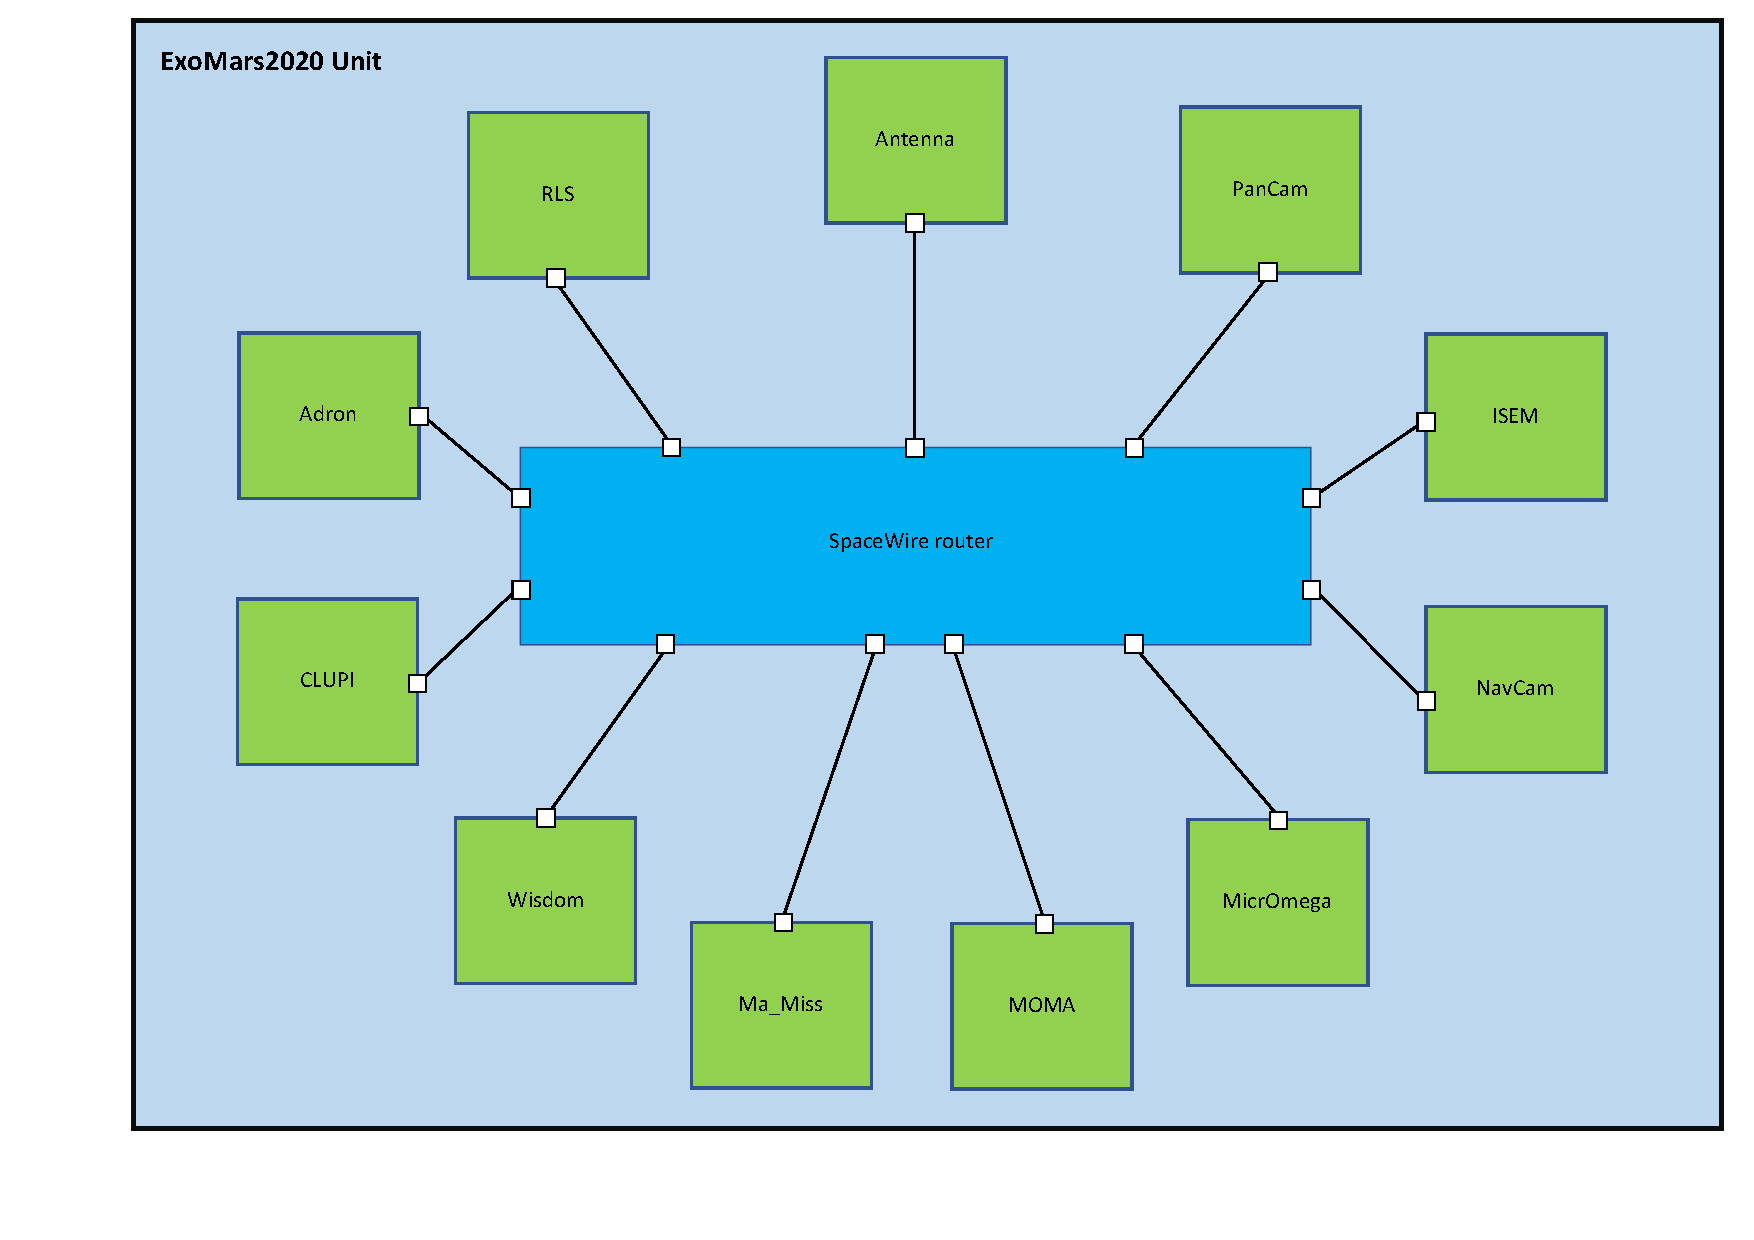
\includegraphics[scale=.5]{pictures/structure_ExoMars2020.pdf}
\caption{Final structure}
\end{figure}
\smallbreak

As in the first task, the SpaceWire Router is modelled by the \Cpp class \texttt{SwitchUnit} and the top module containing all the others by \texttt{NetworkUnit}. But one major difference is that each node is modelled by the same \Cpp class named \texttt{Node}, specialised thanks to a configuration file. This was made in order to avoid boilerplate code, since all nodes have a similar behaviour, errors due to wrong copy of new functionalities in each class, and to prepare the work for a more complex simulator, using a GUI to configure any SpaceWire network.

All details about these improvements will be explained in the following subsections.

\subsection{Features}
Firstly, our project features the modelling of the the third OSI layer of the SpaceWire specification, as requested, but also of a part of the second layer, since it was already done during the first task.
The third OSI layer covers the use of packets to transmit data from one node to another, with possible routing on the way. We modelled only a part of the second layer, since it was kept from the first task and was not mandatory for this one. We only have the transmission by frames of packets, allowing for transmission delay simulations and transmission error modelling (due to some possible incident radiation). It also made us think on the problem of data collision, since we used bidirectional channels, and forced us to create some security mechanism. But we did not implement the Error End of Packet (EEP) and error link recovery at this level.

config files database et processes
\subsection{Network Unit}
\texttt{NetworkUnit} stayed nearly the same since our first task and the corresponding report. It is the module in charge of instantiating all the others and linking them with channels. But its way to do this changed drastically, since we choose to create
\subsection{Node Unit}

It is the module that describes a node, in our case it's the rover's scientific instruments. 

\subsection{Packet Unit}
\subsection{Switch Unit}


\pagebreak

\section{Simulation results}

\subsection{Console output}

ANAS

\subsection{Traces}

ANAS

\subsection{Modelling time comparison}

ANAS

The ExoMars2020 in our project is composed of many several equipment, which are divided into two main parts : the mast and the main body of the rover. The mast can be composed of the PanCam, NavCam, and the ISEM. The main body contains the CLUPI, the Drill, Adron, WISDOM, Ma\_Miss, MicrOmega, RLS, MOMA. Both parts are connected to an antenna which should send information that were gathered to the probe in orbit around Mars, then to the Earth.\smallbreak

Thus, one interesting thing to test and to compare is the modelling time between the simulation of a single model and the one of a parallel model. So, we decided to observe the modelling time of a parallel model that involves the mast part and the main body part working at the same time, and this by creating two processes which are launching two executable that were pre-compiled.\smallbreak

Next, we decided to do a first try by launching a simple simulation, where, every equipment is sending at least one 25-size's packet to another one, and to execute 10 times both model. And, as a result of, we got on average a time execution of $15.46 s$ for the single model, and $15.37 s$ for the parallel model. Then, we do a second try, where this time we send several packets with a consequent size.\smallbreak

\pagebreak

\section{Conclusion}

ANAS

\pagebreak
\nocite{*}
\bibliographystyle{unsrt}
\bibliography{references}

\end{document}